In order to prepare the data acquistion system, the entire electronical chain
was tested beforehand. In fact it is crucial that the response of each
electronic device used behaves linearly, as the information about the energy
of the incident particle must be univocally extracted at the end of the chain.
To test the PROTO Trace detector, it was put in a vacuum chamber, with a α-ray
source.

\subsection{Electronical Chain}

\subsection{GALTRACE Linearity}

\begin{figure}[h]
  \centering
  \begin{minipage}[b]{0.45\textwidth}
    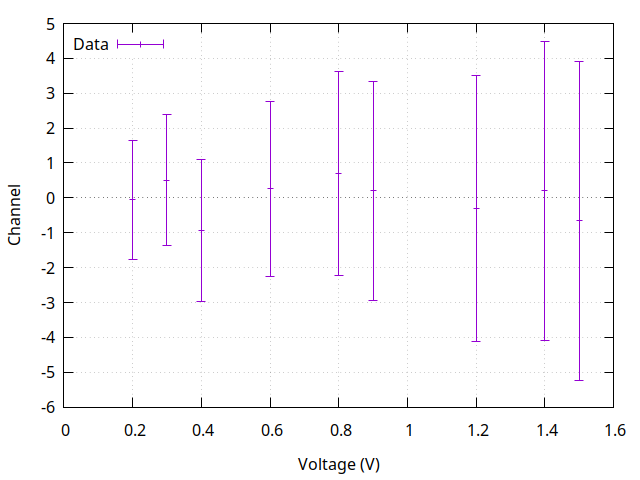
\includegraphics[width=\textwidth]{img/first_board_line/data_2/calib_1.png}
    \caption{Erorr Plot}
    \label{calib:plot:1}
  \end{minipage}
  \hfill
  \begin{minipage}[b]{0.45\textwidth}
  \begin{tabular}{lll}
    Voltage (V) & Channel & $\sigma$ \\
    \midrule
    0.2 & \num{393570.1} & 1.7 \\
    0.3 & \num{393753.2} & 1.8 \\
    0.4 & \num{393934.3} & 2.0 \\
    0.6 & \num{394300.5} & 2.5 \\
    0.8 & \num{394666.1} & 2.9 \\
    0.9 & \num{394848.1} & 3.1 \\
    1.2 & \num{395395.2} & 3.8 \\
    1.4 & \num{395760.8} & 4.3 \\
    1.5 & \num{395942.4} & 4.6 \\
    \bottomrule
  \end{tabular}
  \caption{Data}
  \label{calib:1}
  \end{minipage}
\end{figure}

\subsection{GALTRACE Calibration \& Resolution}

\begin{figure}[h]
  \centering
  \begin{minipage}[b]{0.45\textwidth}
    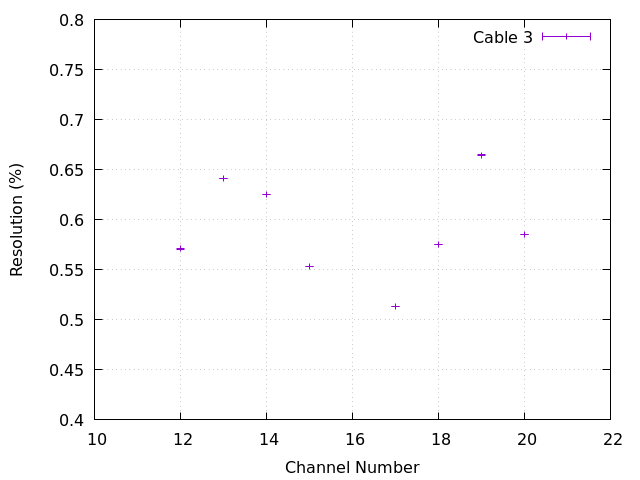
\includegraphics[width=\textwidth]{img/plot/am/3_res_am.png}
    \caption{Resolution vs Channel}
    \label{res:am3}
  \end{minipage}
  \hfill
  \begin{minipage}[b]{0.45\textwidth}
  \begin{tabular}{lll}
    DAQ Channel & Resolution & $\sigma$ \\
    \midrule
    12 & \num{0.5708} & 0.0002 \\
    13 & \num{0.6413} & 0.0003 \\
    14 & \num{0.6253} & 0.0003 \\
    15 & \num{0.5535} & 0.0002 \\
    17 & \num{0.5131} & 0.0002 \\
    18 & \num{0.5752} & 0.0002 \\
    19 & \num{0.6646} & 0.0003 \\
    20 & \num{0.5854} & 0.0002 \\
    \bottomrule
  \end{tabular}
  \caption{Resolution vs Channel plot}
  \label{res:plot:am3}
  \end{minipage}
\end{figure}

\begin{figure}[h]
  \centering
  \begin{minipage}[b]{0.45\textwidth}
    \centering
  \begin{tabular}{ll}
    Channel & FWHM \\
    \midrule
    5150 & \num{29} \\
    5485 & \num{27} \\
    5804 & \num{25} \\
    \bottomrule
  \end{tabular}
  \caption{3-$\alpha$ peaks (cable 1)}
  \label{res:peaks:cab1}
  \end{minipage}
  \hfill
  \begin{minipage}[b]{0.45\textwidth}
    \centering
  \begin{tabular}{ll}
    Channel & FWHM \\
    \midrule
    5153 & \num{32} \\
    5485 & \num{27} \\
    5805 & \num{22} \\
    \bottomrule
  \end{tabular}
  \caption{3-$\alpha$ peaks (cable 2)}
  \label{res:peaks:cab2}
  \end{minipage}
\end{figure}